\section{Idea Analysis}
In November, we put forward the idea of Choona in the PID.  Over time, details have changed and in the section we want to analyse the original idea, the components that make it up and discuss whether or not they remain the same and if not, why have they changed.  

\subsection{The Idea}
We briefly mentioned what Choona was in the introduction.  Its important that we provide a more detailed explanation of the idea and the system behind it.  In order to do this, we will break each section of the project down and briefly explain it.  \\
\textbf{Choona} is the name of our crowd controlled juke box.  It allows users with a mobile device to connect to a Choona location and decide what music they want to listen to.  The name `Choona' came about through word play; \emph{Choone} is a slang term meaning ``a song or any piece of music'' and is related to the word \emph{Tune}.  Tune is quite similar to the word \emph{Tuna} (fish) and a combination of the three words together brought about \emph{Choona}.  The association of the word tuna triggered the idea for the logo; the fish.  Taking it one step further, we tried to integrate technology within the fish which resulted in a WiFi icon styled tail.  This solidifies the idea of Choona; a WiFi icon identifies network connection and Choona will connect a network of people.  In conclusion, a business logo is a method to identify the business and separate the business from its rivals and we believe our logo achieves both. \\

On initial use of the app, the user will be taken to an initial `Welcome' screen.  This will provide details to the user about the main purpose and functionality of the app; to help them understand how to use the app.  Once the user has logged in once, they will never see this screen again and opening the app will take them straight to the login page.  \\

\textbf{Login} - the user will be asked to sign into Choona.  There will different options available to the user; they can log in via a username and password or they can login via a social media account (Facebook, Google+, Twitter etc.).  In essence, this opens up the option for more users to connect quickly and easily with Choona and the opportunity to post on their social media account that they are using this app.  \\

The main reason behind this app is to play the music you want.  Therefore in order to do this, we need a playlist.   This playlist will have several pieces of functionality.  First of all, this will contain the list of songs that have been currently added to the playlist.  The user will be able to scroll this page and look at the different songs.  They can then \textbf{up-vote/down-vote them}.  The idea of the up-vote/down-vote is to push songs further up the playlist so they are played quicker.  Lets consider the example; there is a song that I really like and many other users within the facility also like that song.  If we all decide to up-vote that song, then it will move further up the list because it will have received more votes than other songs on the playlist.  The same is true for the other way; if we down-vote the song, it will move further down the playlist.  This page will allow the user to add songs to the playlist.  There will be \textbf{search} functionality; this explores any connected music source(s) and looks for the song name, artist or album depending on the users input.  Any results will be displayed and the user can add the song they want.  As this is a public system, there will need to be considerations taken on the available music.  There may be occasions when we do not want explicit versions of songs being played (especially when there is a risk of children being present - nightclubs may wish to allow for explicit versions as their customers will be over the age of 18).  Depending on the business and their choice; this will be reflected in the search results and the songs played.\\
In order to stop abuse of the system, there will be a limit on the number of songs a user can add to a playlist at any one time.  There are different options available for this at but we are leaning towards a time-limited based approach.  This would mean that a user can only add e.g. one song every fifteen minutes.  It has been suggested that we add a points system to this facility that allows you to gain points through the number of up-votes any of your previously added songs receive.  Once you get over a certain amount of points, the number of songs you can listen to is bumped up.  
There may be instances when no songs have been added to the playlist by users.  If this is the case, there will be a \textbf{default playlist} available that kicks in when the user playlist becomes empty.  This means that there won't be any stage when there is no music being played.  This default playlist is created and maintained by the business through their Choona account.  Now we have the playlist, how do we connect to it?\\

Different locations will have different playlists.  In order to differentiate between these distinct locations, we will make use of \textbf{Geolocation}.  There are two sides to this; the business will have to have to create a boundary - this would be their shop floor area.  We call this a \emph{Geofence} and it acts like a virtual barrier.  When inside the barrier, the user will have access/connection but when they leave, the user looses their access/connection.  The second part to this is the mobile device.  Using the locations services available on mobile devices, we can then determine whether they are inside the geofence.  This therefore means we can allow customers to connect to that locations playlist where they can then add their own song choices and up-vote/down-vote other song choices on the playlist.  
Using this functionality, we can also make sure the state of the playlist is ideal for the current users.  If a user leaves the geofence; any song(s) they have added to the list can be removed if that song(s) has not received any up-votes from any other users. \\

As we mentioned earlier, Choona allows for social media login but we take this one step further.  We want to use social media as a way of socialising with friend.  We have decided to use a notification system where users can add posts from Choona onto their social media account.  A post will contain location (through geolocation), the song currently being played and a timestamp; something like ``Chris is listening to Happy by Pharrell Williams at Loughborough Students Union - 10 minutes ago''.    In the app itself, any notifications posted by friends that are Choona users will be displayed.  This is a small simple but fun aspect to the app and has been introduced because teenagers and young adults in todays society are heavy social media users with a large social influence.  \\

Within the app, there will be a \textbf{history} page.  Within this history page, there will be a list of different Choona locations that you have connected to.  Behind each of these locations, there will be a list of songs that were played from when you entered that geofence to when you left the geofence.  With this functionality, we are trying to provide the user with the ability to check back and find a song that they really liked but do not know the name of.  It is a regular occurrence they we listen to a song but do not know what it is.  With background music, it is hard to use an app like ``Shazam'' or ``Soundhound'' to identify the song for two reasons; the volume is too low or there is too much noise to identify the song.  Therefore the history feature on Choona can allow the user to find out what that song is.  Further to this, there will be functionality to \textbf{purchase or play} that song.  Choona will look at the different music providers on the mobile device and then offer the option for the user to connect to that provider and play/buy the song e.g. if running Spotify, the app will offer the option to ``Play in Spotify'' thus allowing the user to add that song to their own private music collection.  \\

There may be environments when you want to listen to the music but there is too much background noise.  This can be common for customers in coffee shops who are there to work or for people in an office environment.  Choona will enable the user to listen to the playlist privately; through the use of headphones.  Very simple and could be very effective.  \\

There would be two different types of Choona accounts; standard user and admin.  The customer will sign up for the standard user account, providing them with the functionality described above.  The admin account is the account provided to the business.  This is used for the purposes of identifying the music sources.  The admin account will link up with the different available music sources to that business.  This is linked to the search functionality in the customer app so the search results that appear for the customer relate to the music available from the connected source.  Furthermore, the admin account will deal with adverts.  The Choona app allows for advertising in two forms.  The first within the app; at the top of the playlist, there will be an accordion.  Within this accordion, the admin can either have one single image; depicting the business or they could utilise it for the purposes of adverts.  They can place multiple different images that scroll through with each one depicting whatever they want; a new product or a special offer.  The second form of advertising comes in sound bites.  These sound bites would be positioned between songs (this is handled automatically by the Choona system).  The admin account will just have to add the sound bites they want to placed between the songs.  

\subsection{Use cases}
We have created a few different use case examples to help solidify the idea of Choona.
\subsubsection{Coffee Shop} 
Choona would connect with the current audio output in the coffee shop and through either the mobile app or the web interface, customers can decide what music they listen to.  \\

    \begin{figure}[h!]
      \centering
      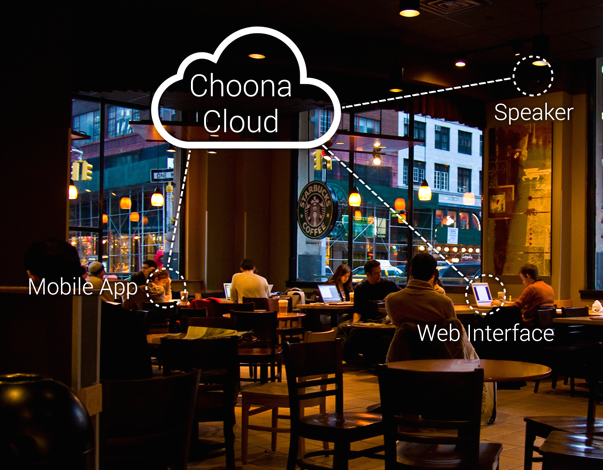
\includegraphics[width=0.8\textwidth]{./img/coffee-shop.png}
      \caption{Coffee Shop Use Case}
      \label{fig:coffee_shop}
    \end{figure}

\subsubsection{Night Club} 
In a night club, Choona becomes a system where users can choose the music they want to hear.  These results are passed to the DJ through the custom adaptor and they can customise the music to match the crowds preference(s).  \\

    \begin{figure}[h!]
      \centering
      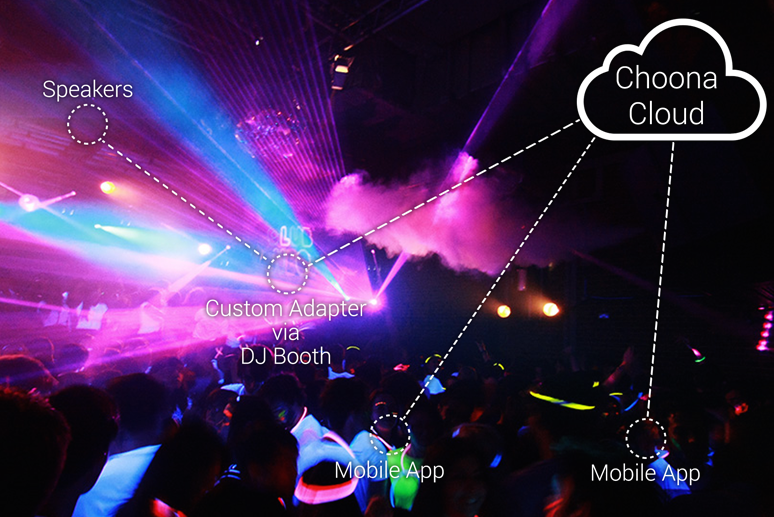
\includegraphics[width=0.8\textwidth]{./img/nightclub.png}
      \caption{Night Club Use Case}
      \label{fig:night_club}
    \end{figure}

\subsubsection{The Office} 
In the office, Choona plays the songs chosen by the employees.  There are two different wasy to listen to the music here; via the speakers or via headphones.  Choona will allow users to put headphones on and listen to the music privately via their mobile device. \\

    \begin{figure}[h!]
      \centering
      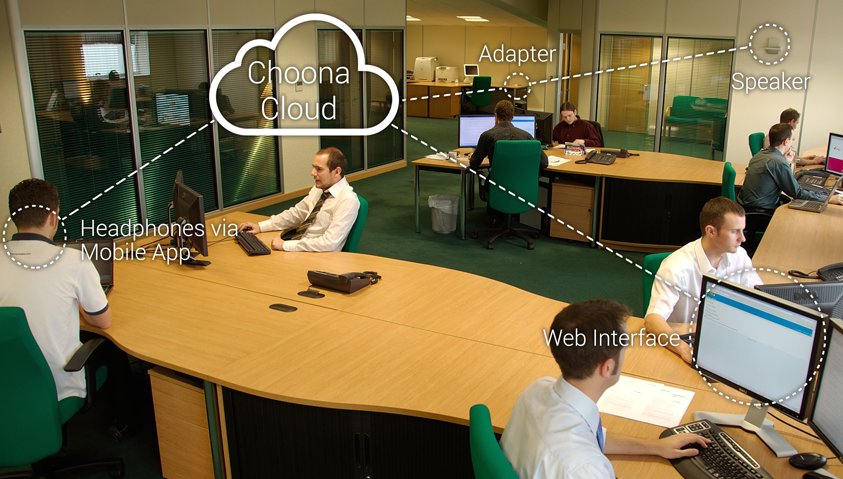
\includegraphics[width=0.8\textwidth]{./img/office.png}
      \caption{Office Use Case}
      \label{fig:office}
    \end{figure}

\subsection{User Value Proposition}
There are four small sections that curtail a value proposition.  These have been outlined below:
\begin{itemize}
\item \textbf{(1)} Headline - one short sentence about the end-benefit we are offering
\item \textbf{(2)} Small paragraph - explanation of what we offer, for whom and why its useful
\item \textbf{(3)} Key benefits and features of the app
\item \textbf{(4)} One visual - pictures paint a thousand words
\end{itemize}
Based on the criteria above, we have written the follow proposition.\\

\textbf{(1)} Choona is a music-sharing app allowing users to collaboratively listen, interact and suggest music in public areas, businesses or homes through an intelligent, cloud-driven system.  \\

\textbf{(2)} This app is for anyone who wants a say in the music they listen to; users can access music playlists through geolocation and add the songs (from different sources) they want.  Songs move further up the playlist the more ``up-votes'' they receive or further down the queue the more ``down-votes'' they receive.  Choona offers social media interaction and provides a catalog of history to help find the song(s) thats name you can't remember.  \\

\textbf{(3)} There are several key benefits to Choona for the user:
\begin{itemize}
\item Listen to your preferred music - In too many situations, we are forced to listen to music that doesn't interest us.  Though the majority of times the music is in the background, we somehow know it's there.  If we enjoy that music or can relate to that music in any way, it has a positive effect on our attitude and what we see.
\item You do not need to sign up; you can log in using a social media account.
\item Adverts can help highlight a new range of products or identify any special offers that you may be interested in.
\item Helps identify songs that you cannot remember the name of or the artist that sings it.
\end{itemize} 

\textbf{(4)}\\
\begin{minipage}{\linewidth}
\centering
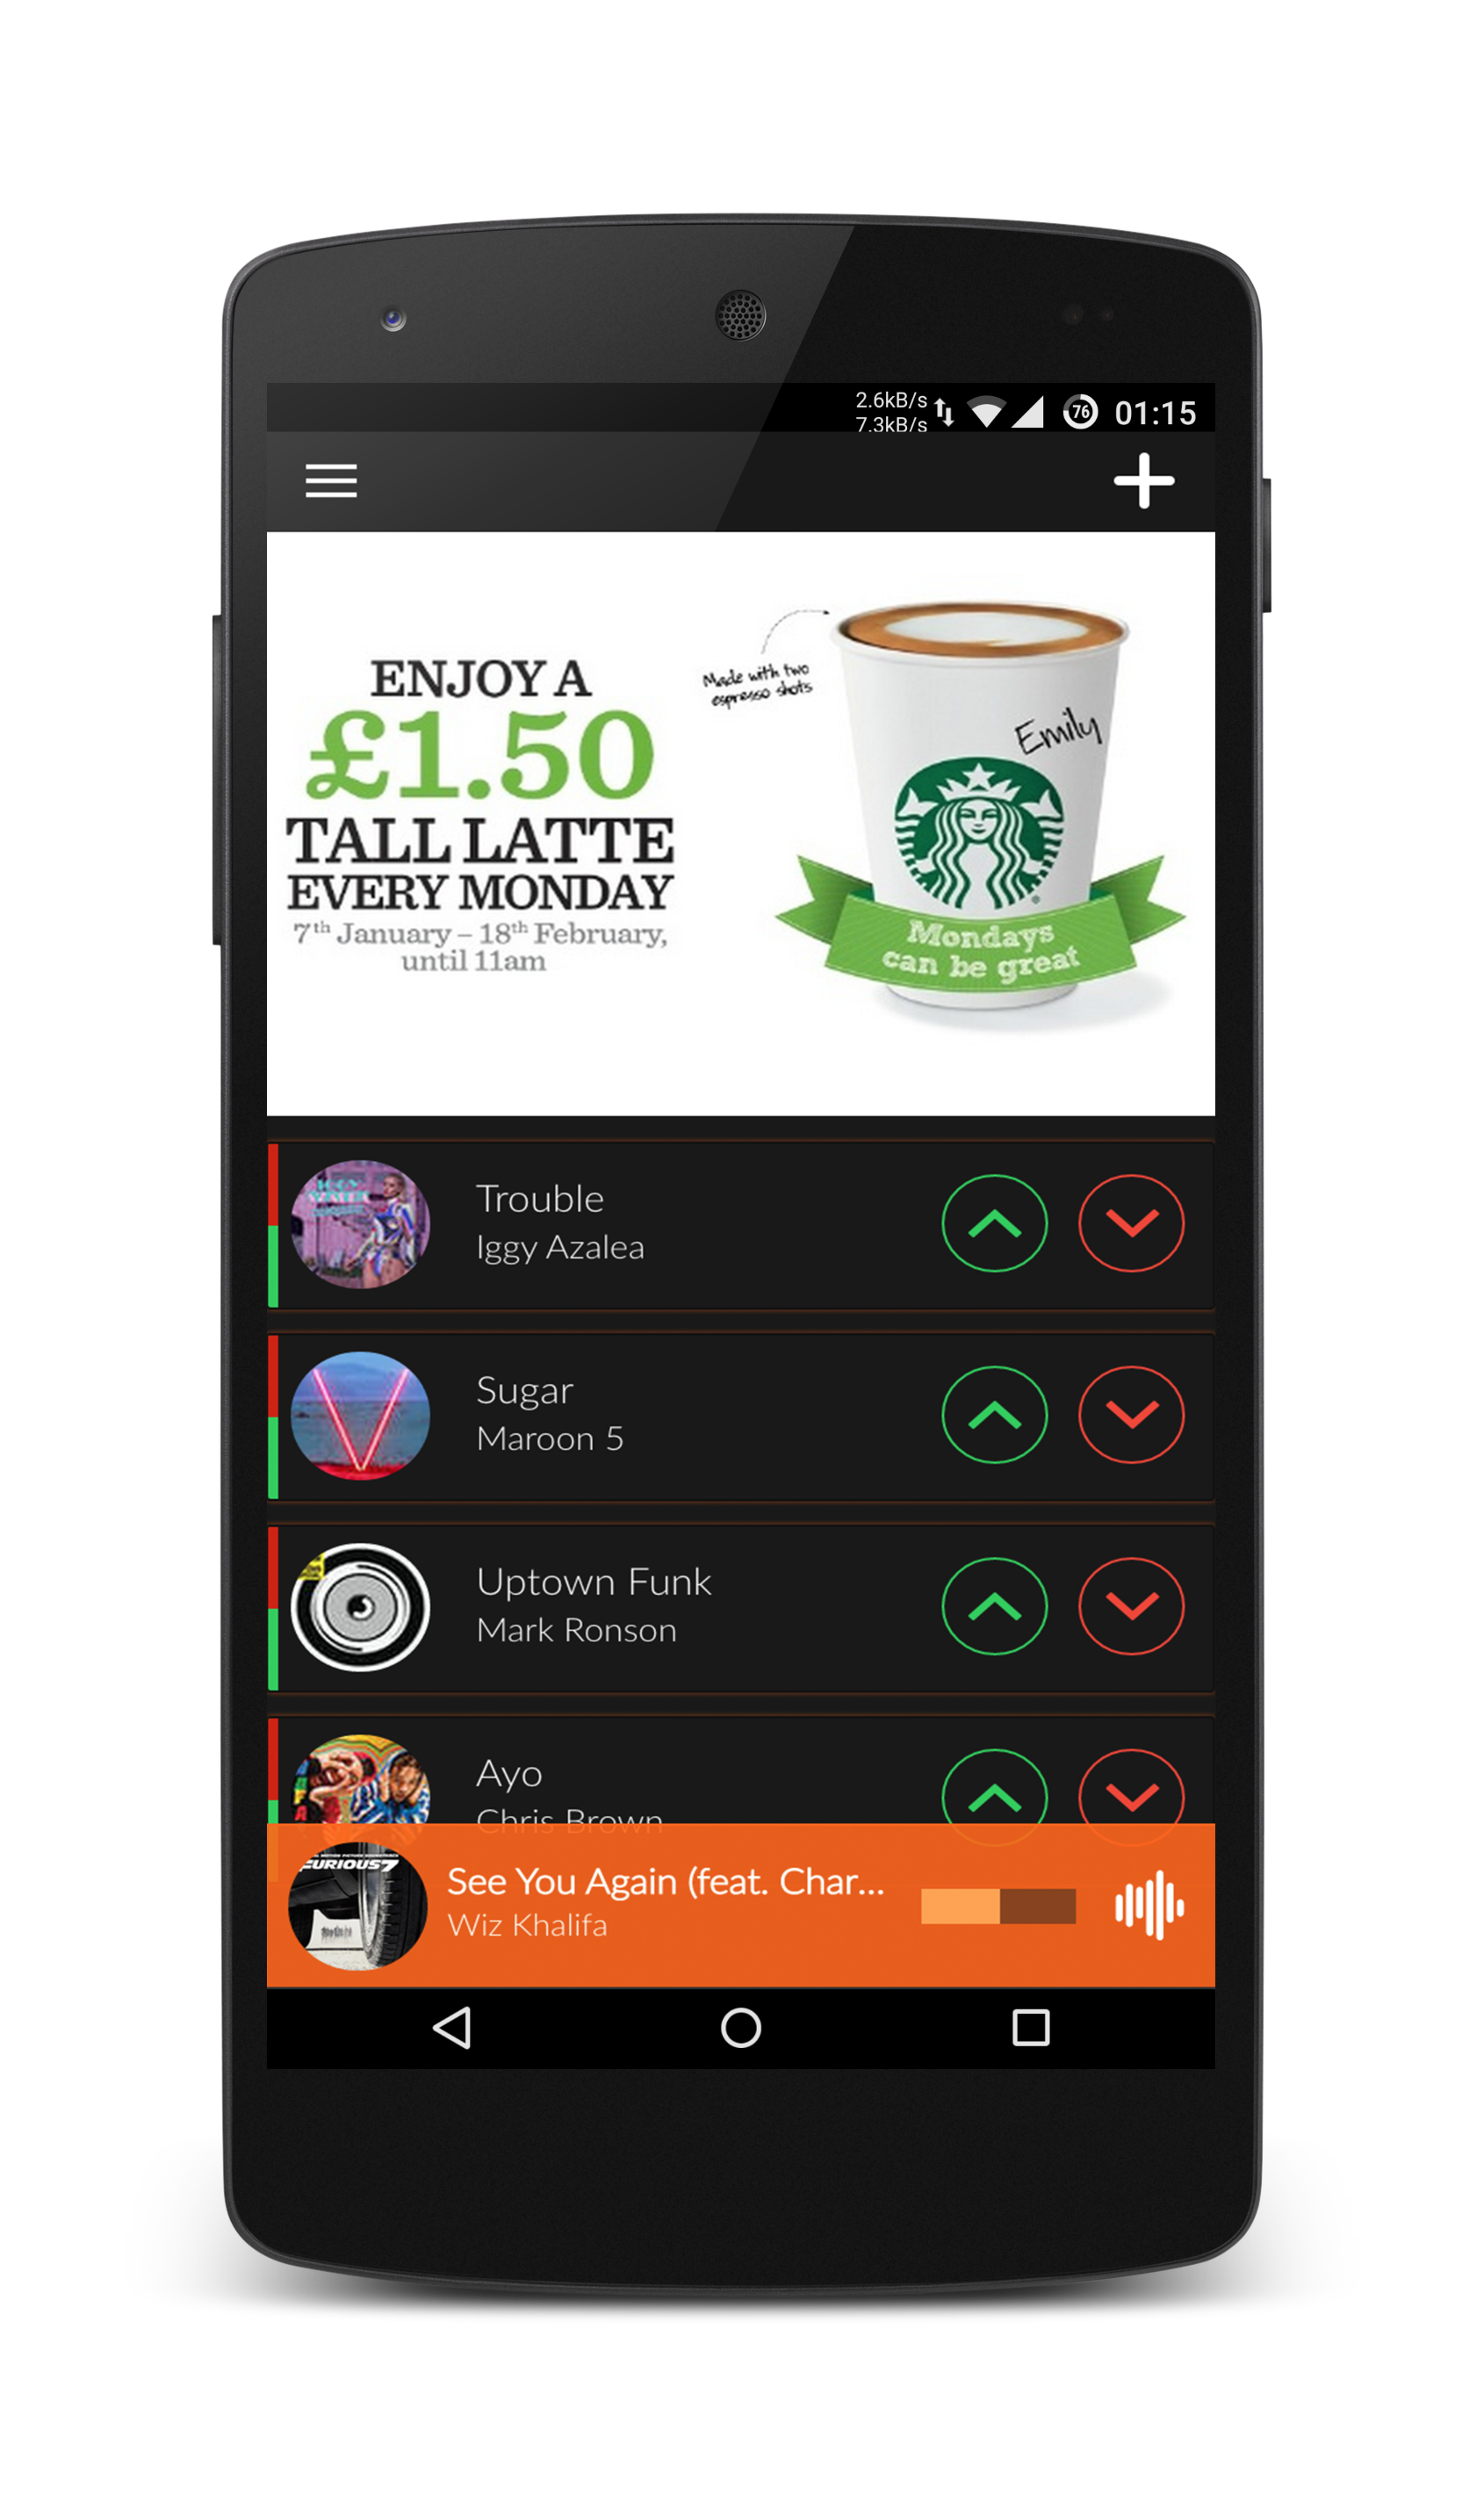
\includegraphics[width=0.3\textwidth]{./img/idea_user_prop.png}
\captionof{figure}{This is the playlist part of the app where users can add their favourite songs as well as up-vote and down-vote any songs within the playlist.}
\label{fig:image_user_prop}
\end{minipage}\\

\subsection{Business Value Proposition}
We have carried out a value proposition for the business and this follows the same structure as the user value proposal.\\

\textbf{(1)} Choona is a music-sharing app that allows customers to collaboratively listen, interact and suggest music in your retail space or business premises through the cloud-driven system.  \\

\textbf{(2)} Choona offers the business a way to enhance a customers experience.  Allowing customers to listen to their favourite music is a sure way of making sure they stay longer and that they make more purchases.  It is also a great way to advertise (via images and sound bites) new products and special offers that may otherwise go unnoticed.  \\

\textbf{(3)} There are several key benefits to Choona for the business:
\begin{itemize}
\item Customers may stay longer thus increasing the number of purchases they make; this increases sales and profit.
\item Advertisments will also gain increased product interest and increased sales revenue
\item Data analytics - Choona will collect endless amounts of data that can then be analysed to find trends or relationships that help the business improve in any area it wants/needs.  
\item The business has an increased/new online presence through the social media activity feature. 
\item Businesses can taylor their default playlist to music that suits their target audience thus making sure they attract the right customers.
\end{itemize} 

\textbf{(4)}\\
\begin{minipage}{\linewidth}
\centering
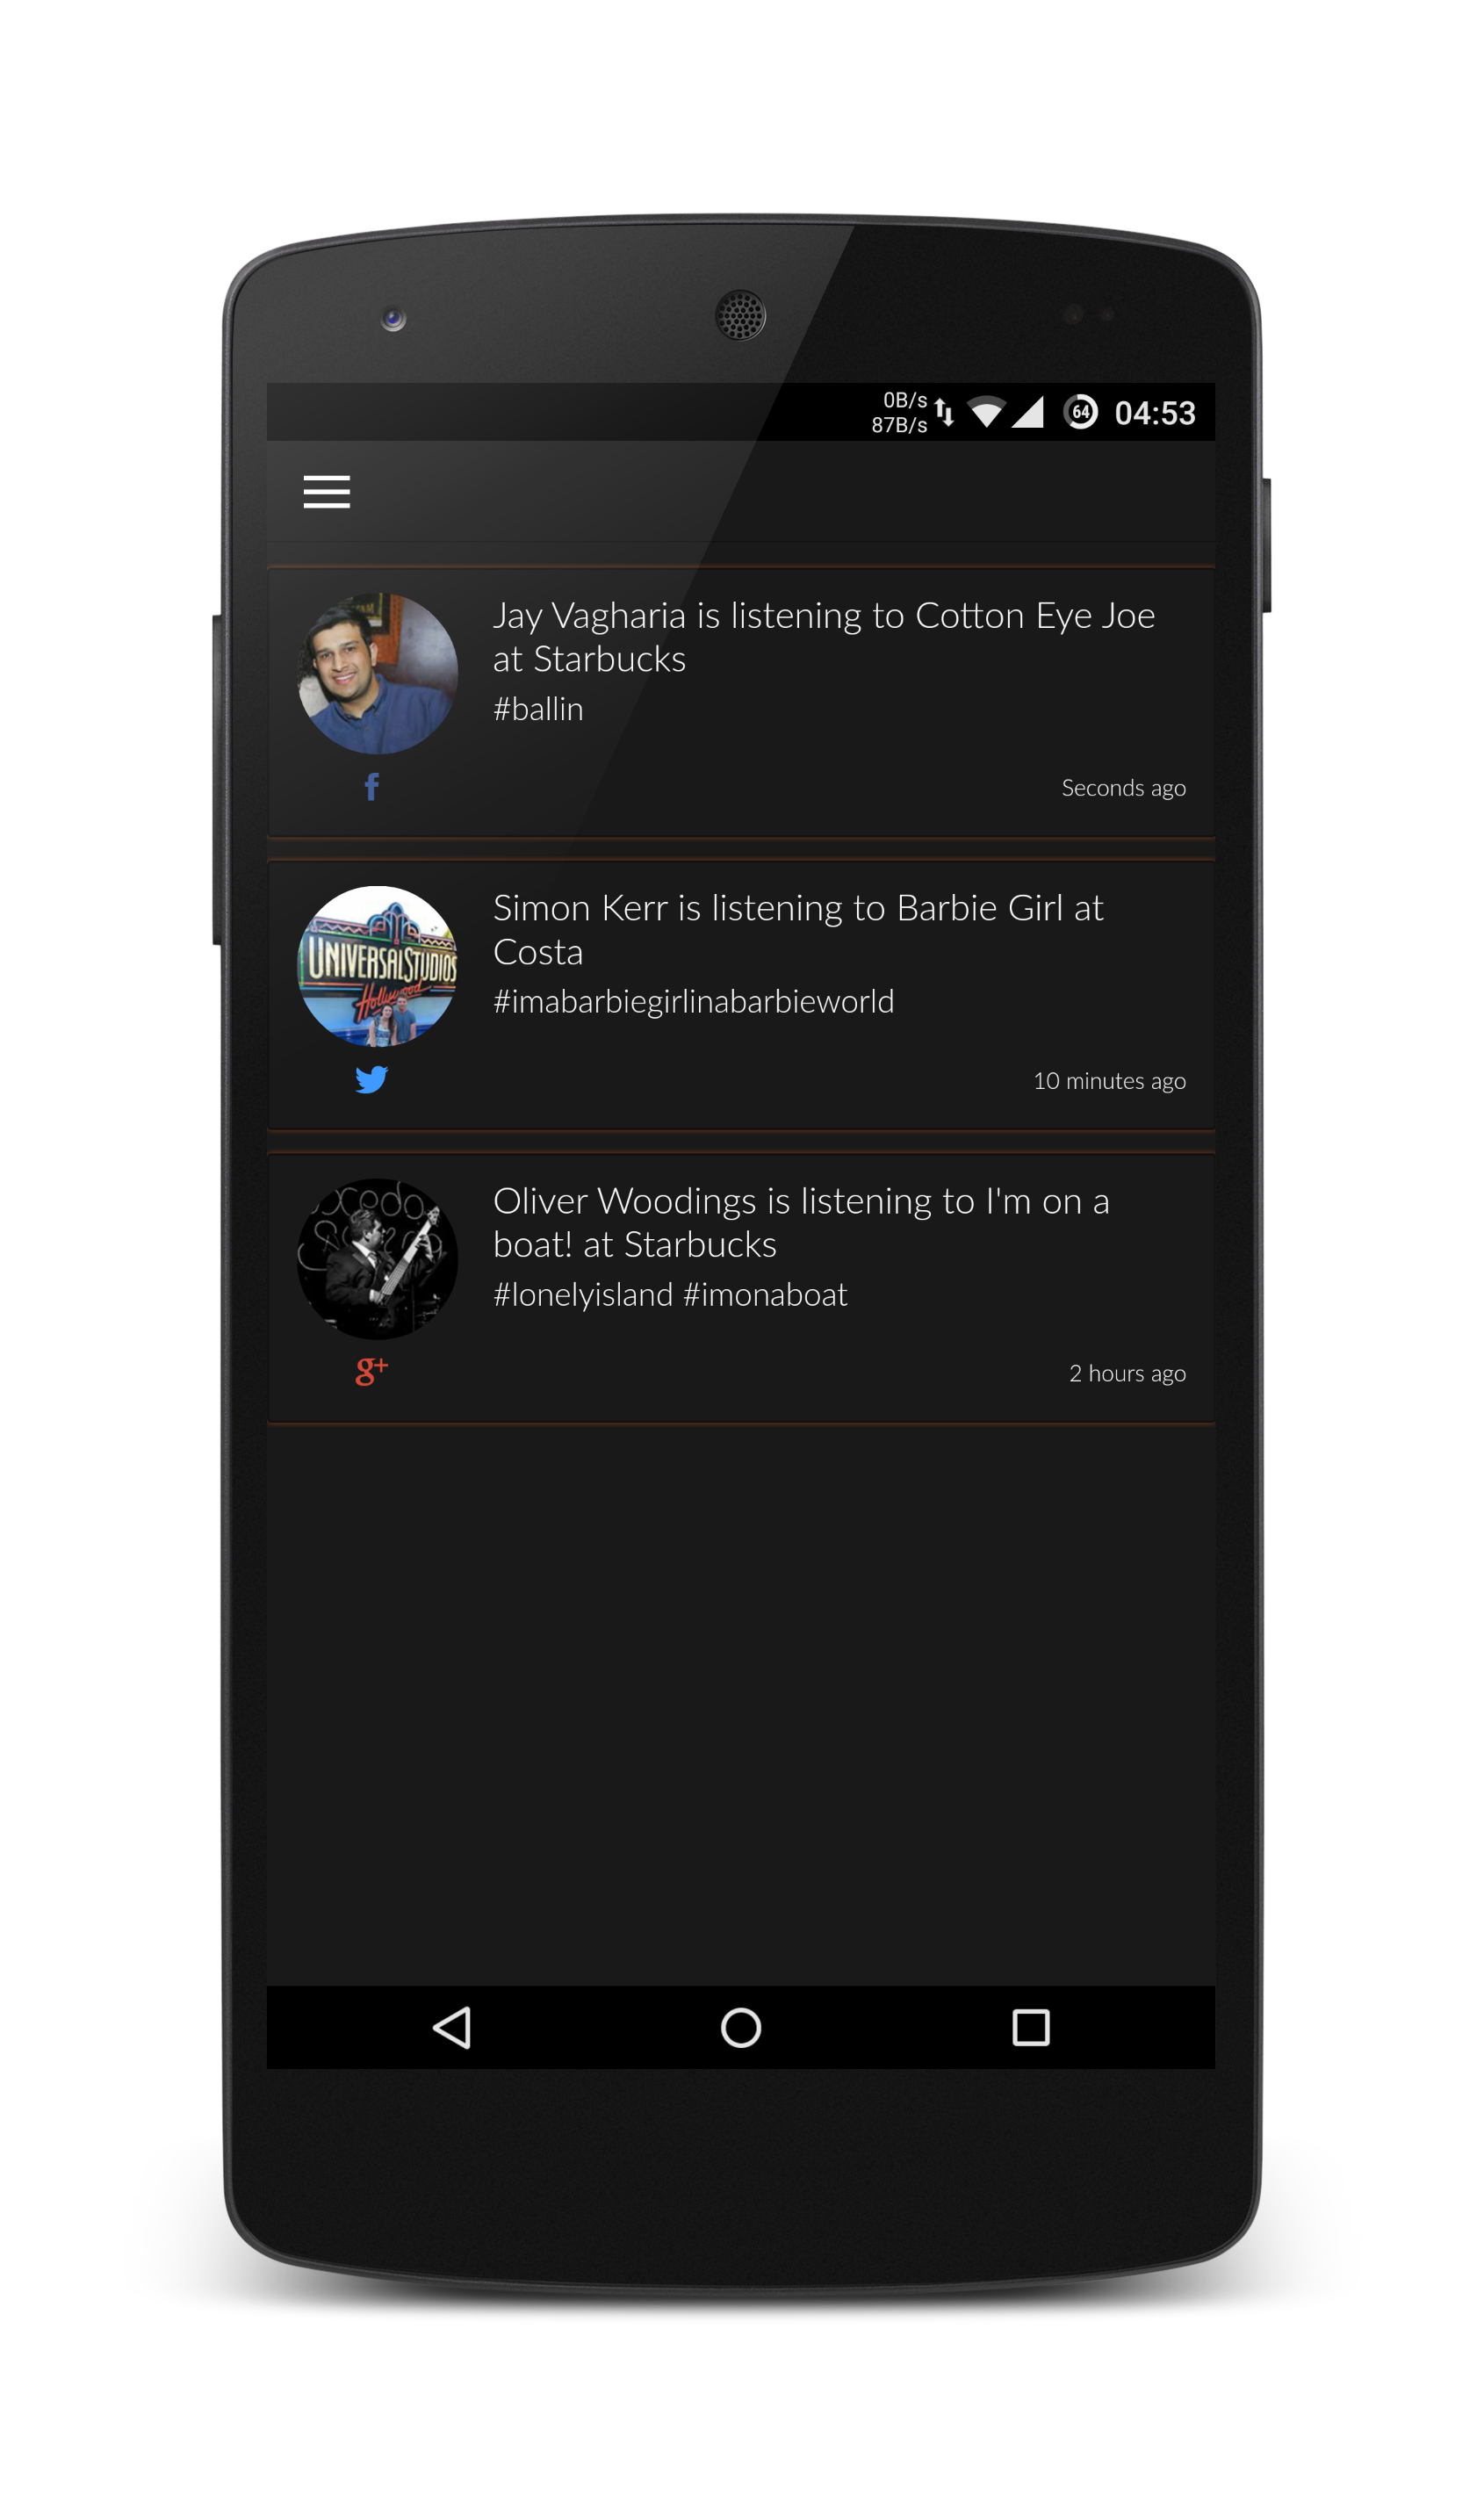
\includegraphics[width=0.3\textwidth]{./img/idea_bus_prop.png}
\captionof{figure}{This is the activity page; this is where the online presence of the business starts to grow.  Please refer to figure ~\ref{fig:image_user_prop} for a look at the placement of image adverts.}
\label{fig:image_bus_prop}
\end{minipage}\\

\subsection{Business Model}
As part of the business plan, we created a lean canvas.  This is shown below; and depicts how we aim to bring success with Choona.\\

\noindent\makebox[\textwidth][c]{%
\begin{minipage}{\linewidth}
\centering
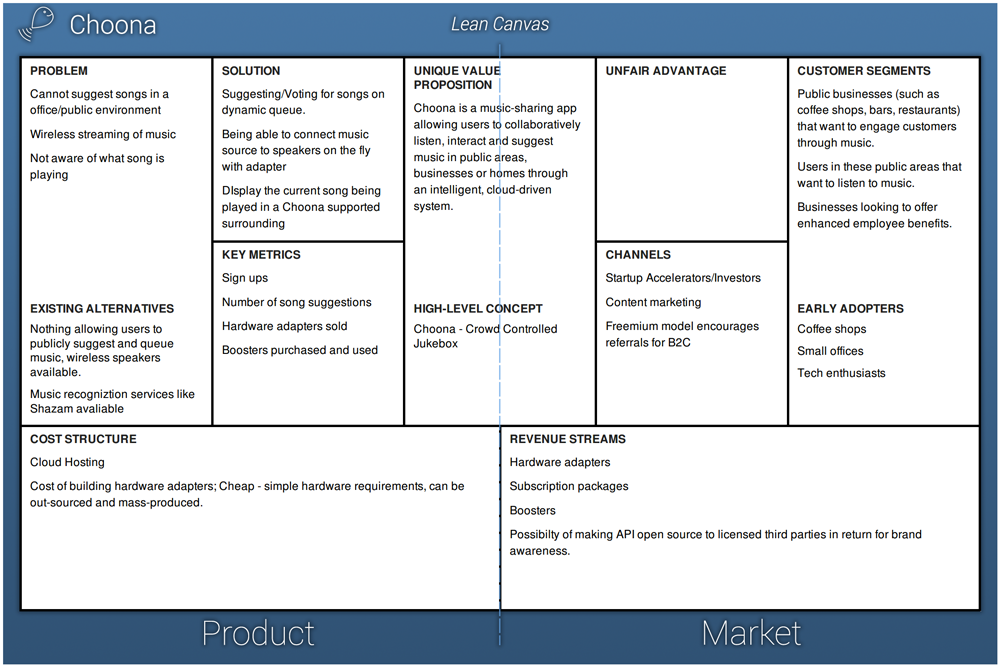
\includegraphics[width=1.0\textwidth]{./img/lean-canvas.png}
\captionof{figure}{This lean canvas has taken inspiration from Peter Drucker and his theories on firms as well as aspects of Michael Porter's value chain maps.}
\label{fig:lean_canvas}
\end{minipage}}\\

\subsubsection{The problem solved?}
At the moment, there is no service that provides users with the ability to select the music they listen to in public areas and the office.  Choona provides them with this ability through a simple mobile facing app that interacts with a system connected to the cloud.   \\

\subsubsection{B2B}
The B2B model essentially means we are providing a product or service to a business.  We are providing businesses with the ability to offer Choona to their customers.  An administration account will be provided that finds their music source(s) and makes it available for customer access.  This account will be allocated a certain number of user connections based upon the subscription package they purchase.  The business will have access to define a default playlist; playing when no other songs have been added by customers.  Businesses will also be able to advertise to customers, whether it be via images on the customer facing app or via sound bites that are inserted between songs.  \\
There will be several different subscription packages available for the business to subscribe to.  The larger the business (whether that be across one location or multiple locations), the more connections they will want to have.  A large organisation will have two levels of management; management across the overall Choona account and management for each different Choona location.  Regardless of this, there will be a standard offering of packages and these are outlined in figure ~\ref{fig:sub_packages}.  \\

\noindent\makebox[\textwidth][c]{%
\begin{minipage}{\linewidth}
\centering
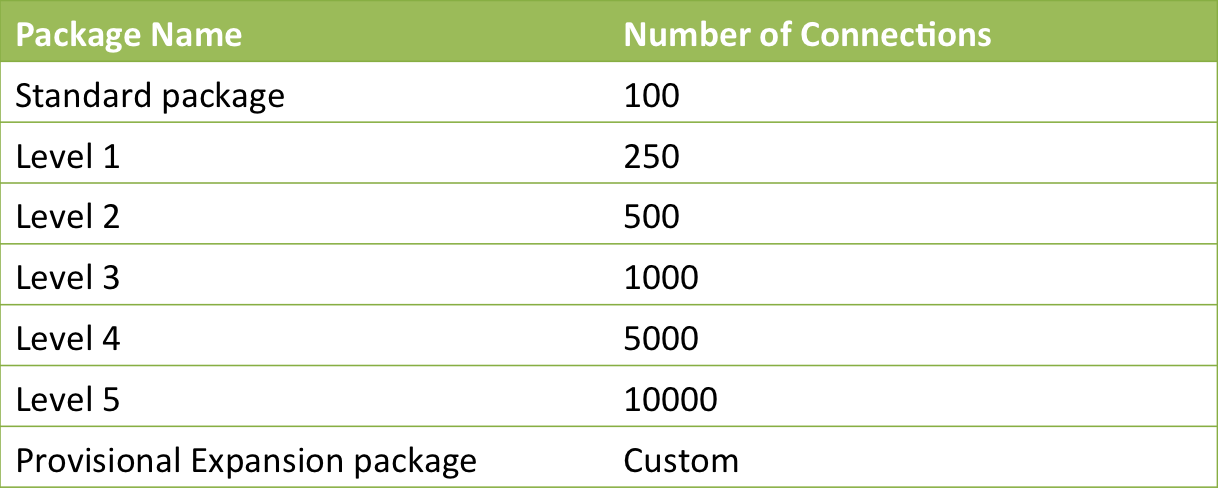
\includegraphics[width=0.8\textwidth]{./img/b2b.png}
\captionof{figure}{Subscription packages}
\label{fig:sub_packages}
\end{minipage}}\\

Unfortunately, we have not had enough time to carry out cost analysis and therefore we cannot put a price beside these packages.  A detailed research analysis of the market will have to be carried out before we can make such estimations.  We do however have a outline on what each package offers; number of connections.  The standard package is a very small package and is aimed at small businesses.  This will be a free package as we plan to adopt a freemium model.  A freemium model is one where core functionality is given away for free but the premium product is sold for a price.  The reason behind using this approach is that it should promote brand awareness and entice more businesses to offer Choona and entice more customers to use it.  \\
In the B2B model, a small number of connections will be given away but in order for the business to allow more customers to use the service, they will have to pay for any additional connections (through upgrading their packages).  The premium packages move from Level 1 to Level 5 and range from 250 connections to 10000 connections. These packages have been created based on several different sources and the information they have provided.  Firstly, according to business insider, Starbucks have around 625 customers per day per store\footcite{starbucks} across 750 stores in the UK\footcite{starbucks_more}.  Therefore, across the UK per hour, they are server over 43000 customers.  This is a huge number and therefore a large connection package would be needed to offer Choona to all customer.  This is why we have created Level 5 package.  Based upon the figures from JS Sainsburys\footcite{sainsburys}, they carry out around 119 transactions per hour per store.  This is a significant number and with more than 1200 stores across the UK, they too need a large number of connections.  We have also spoken to a member of the Loughborough Students Union.  On hearsay, they have estimated the average number of people on a night out to be around 4500.  Over the course of a 6 hour night, this would fluctuate somewhat but at anyone time, the average number of customer would remain around 2000 people.  This has resulted in package levels 3 and 4.  Packages 1 and two have been created for the purposes of smaller businesses that have one, maybe two locations and for large businesses that would use Choona as an internal music application.  Provisional expansion packages are for the one-off occasions where it is not necessary to have the package for a specific length of time.  Concerts are a great example, they happen over a 1, 2 or 3 day period.  Rather than miss out on the Choona experience, we can offer a package that matches the event in terms of duration and number of connections; its a win-win for both the business and for Choona.\\
The second part to the premium side of the freemium model is the sale of a physical adaptor.  This can be purchased as another method of connecting to the cloud and streaming music.  Businesses may want to purchase such hardware whenever laptops and computers are not readily available. \\

\subsubsection{B2C}
B2C covers the private use of Choona within one location and for a non-commercial use.  This covers private parties and normal day to day use between yourself and immediate family within the home.  The B2C model is similar to the B2B model in that it will follow the freemium model.  The user will have free access to the Choona app where they can use it in different Choona locations.  Whenever they want to privatise and create their own Choona location, they have to subscribe for a standard package; this will be free.  However this offers a very small number of connections (5).  If they wish to increase their number of connections, they can upgrade to a higher package.  At this moment in time, we have not been able to do any research towards this type of subscription and therefore we cannot outline package levels or number of connections within these packages.  \\

\subsubsection{Subscription Model}
As we identified in both the B2B and B2C models, we will adopt \emph{subscription commerce}.  On a monthly/yearly basis, the businesses subscription will be renewed and a fee will be paid to Choona.  There are numerous benefits for adopting such a model.  For the business, they will never have to remember to reorder every month; which provides them with the piece of mind that they will receive exactly what they have signed up for.  It is also good for Choona as this will provide us with a constant revenue stream.  We won't need to be constantly bring them through a `checkout' process. 
Secondly, subscription based services are generally a novel idea within their market.  The novelty alone will create a good deal of publicity and drive sales without the need for large volumes of publicity.  \\
It is important to consider the subscription length because a longer average will increase the Customer Lifetime Value.  In doing so, Choona will maintain an increased profitability rate due to the retention of customers and businesses.  This will result in us being able to pay more (through advertising and personalised subscription packages) to sign up further businesses and customers.\\
